\documentclass[11pt,a4paper]{article}
\usepackage[margin=1in]{geometry}
\usepackage{amsmath,amssymb}
\usepackage{booktabs}
\usepackage{graphicx}
\usepackage{longtable}
\usepackage[round,authoryear]{natbib}
\usepackage{hyperref}
\hypersetup{colorlinks=true,linkcolor=blue,urlcolor=blue,citecolor=blue}

\title{An Empty Region of Technical Strategy Space:\\
18{,}630 Pre-Registered Variants Across Cryptocurrency and FX}

\author{Mobin Moharami\\
\small Independent researcher\\
\small \texttt{mobin@greencandle.vc}}

\date{October 2026}

\begin{document}
\maketitle

\begin{abstract}
Published results about trading strategies pass through a filter that keeps
only what worked. This paper reports the other side of that filter. Seventeen
strategy families were enumerated exhaustively into 18{,}630 parameter
variants and evaluated on hourly cryptocurrency and FX data. Every sweep was
pre-registered: the search space, protocol, cost model and acceptance
threshold were written down, hashed with SHA-256, and anchored to the Bitcoin
blockchain before the corresponding data was loaded. The full return
distribution of every variant is reported, not the best one.

Across 29 scored sweeps, none cleared a Deflated Sharpe Ratio of 0.95. The
highest observed was 0.745. In 27 of the 29 sweeps the best variant performed
worse than the maximum expected under the null hypothesis of no skill --- that
is, worse than the best of an equivalent number of random strategies. The
median minimum detectable annualised Sharpe was 3.49, which bounds what this
study could and could not have seen: effects below that threshold remain
untested rather than refuted.

Four results follow from reporting every sweep rather than the best one. A
sign test across sweeps rejects the joint null of no effect in the direction
opposite to the one a reader might expect ($p = 1.6\times10^{-6}$): the
families underperform chance collectively, not merely individually. A
cost-sensitivity decomposition separates families that die under transaction
costs from the seventeen of twenty-nine whose median variant is unprofitable
even at zero cost. The measured kurtosis of the realised return series
exceeded the value assumed at pre-registration in every single sweep, by a
median factor of 354. And the two cross-sectional momentum sweeps produced
positive gross Sharpe in every one of their 45 variants, with a median
breakeven cost of 29 to 31 basis points against the 10 charged, while
remaining inside the spread of independently shuffled panels ($z = 0.8$ and
$1.8$) and below the acceptance threshold --- a case where two independent
criteria, one analytic and one empirical, agree that an apparent effect cannot
be separated from noise.

The registry also records its own failures. Three cross-sectional sweeps were
voided before submission, when a weight-allocation defect
was found that assigned the entire short leg of half their variants to assets
outside the investable universe. They were re-registered, re-timestamped and
re-run; both the voided records and their replacements are reported here. One
of the three replacements is the exact arithmetic inverse of another and is
marked as one piece of evidence rather than two.

The contribution is not a claim that technical trading does not work. It is a
mapped region of strategy space with a stated detection limit, published
whether or not it contained anything, together with the timestamps that let a
third party verify the pre-registration independently of the author. Every
sweep, including the eight that were voided and the reasons for voiding them,
is reported in the appendix.
\end{abstract}

\section{Introduction}

Consider a thousand researchers independently testing the same worthless
strategy. Roughly fifty will observe a result significant at the five percent
level. If only those fifty publish, the literature will contain fifty
confirmations and no refutations, and a reader cannot distinguish that
situation from one in which the strategy works.

This is not a hypothetical concern in quantitative finance. Backtests are
cheap, the space of testable rules is effectively unbounded, and the incentive
to report only the surviving variant is strong. \citet{bailey2014} showed that
with enough trials a backtest with an in-sample Sharpe ratio of 1.0 can be
produced from pure noise, and derived the Deflated Sharpe Ratio to correct for
it. \citet{harvey2016} argued that most published cross-sectional return
predictors fail once multiple testing is accounted for.
\citet{lopezdeprado2018} described backtest overfitting as the central
methodological problem of the field.

The corrections exist. What is missing is the negative record: systematic
publication of regions that were searched and found empty. Without it, the
corrections are applied to a sample that has already been filtered.

This paper reports one such region. It is small relative to the space of
possible strategies, and the result will not surprise anyone who has
internalised the multiple-testing literature. Its value is that the search
space, the protocol and the threshold were fixed and cryptographically
timestamped before the data was examined, so the absence of a positive result
cannot be attributed to a threshold chosen after the fact.

\section{Method}

\subsection{The unit of publication}

The unit here is not a strategy but a \emph{region of strategy space}. The
statement ``RSI(14) did not work on BTC'' carries almost no information: it
describes one point in a continuum, and the reader cannot tell whether a
neighbouring parameter would have worked. The statement ``the entire
short-horizon mean reversion family, 1{,}620 enumerated variants, across two
symbols over eight years, produced nothing above a stated detection limit'' is
a claim someone else can build on or refute.

Every sweep therefore enumerates a complete parameter grid rather than
selecting parameters. No variant is favoured, and the whole distribution is
reported.

\subsection{Pre-registration and timestamping}

For each sweep a JSON document was written specifying the strategy family and
its full parameter grid; the symbols, timeframe and date range; the execution
and cost model; the planning assumptions used for the power calculation; and
the acceptance threshold. The document was canonicalised, hashed with
SHA-256, and the hash submitted to OpenTimestamps~\citep{ots}, which anchors
it in a Bitcoin transaction.

The ordering this establishes is the point. A reader can verify that the
document existed in its current form before the block containing its hash was
mined, and therefore before any result reported here. Only the hash is
published to the timestamping service; the document itself stays with the
author until release.

All 38 pre-registrations in the registry carry such a timestamp.

Records are additionally linked in a hash chain,
\begin{equation*}
\mathrm{chain}_i = \mathrm{sha256}\!\left(\mathrm{chain}_{i-1} \,\|\,
\mathrm{id}_i \,\|\, \mathrm{sha256}(\mathrm{prereg}_i)\right),
\end{equation*}
with $\mathrm{chain}_0 = \mathrm{sha256}(\texttt{"sweep-registry-genesis"})$.
Timestamping alone proves that each document predates its result but says
nothing about deletion: an inconvenient record could be removed quietly and
every remaining one would still verify. Under the chain, removing a record
changes every subsequent link, including the published head. For a registry
whose contents are almost entirely negative results, that is the failure mode
worth defending against.

\subsection{Implementation}

Each variant maps a signal to a target weight at the close of bar $t$, held
over bar $t+1$. Signals are computed only from information available at or
before the close of $t$; no indicator uses a centred window, and no
rebalance uses the bar it is executed in. Within a sweep every variant sees
the same bars, so cross-variant comparisons are not contaminated by differing
sample lengths.

Costs are charged on the absolute change in weight,
\begin{equation*}
r_t^{\text{net}} = w_{t-1} r_t - c\,\lvert w_{t-1} - w_{t-2} \rvert ,
\end{equation*}
where $c$ is the round-trip cost in basis points fixed at pre-registration
and never adjusted after seeing a result: 4~bps commission plus 6~bps
slippage for the cross-sectional sweeps, which trade altcoins outside the
majors and for SW-0036; 4 plus 2 for the other single-asset crypto sweeps;
and 1 plus 0.5 for the
FX sweeps, where major-pair spreads are a fraction of those in crypto. The
lower FX charge means a smaller true edge would have survived there, so a
null result on FX is stronger evidence than a null on crypto, not weaker.

Sharpe ratios are annualised as $\sqrt{P}\,\bar r / s_r$ with $P = 8{,}760$,
the number of periods per year declared in every pre-registration. For the FX
sweeps this treats the five-day trading week as if it were continuous, which
inflates the annualisation factor by roughly 18\%; the same constant is
applied to every variant within a sweep, so cross-variant comparisons and the
sign of each result are unaffected, but the FX Sharpe levels reported here are
not directly comparable to figures annualised on a 252-day convention. No risk-free
rate is subtracted; over this sample the adjustment is small relative to the
dispersion across variants, and omitting it is conservative in the sense that
it inflates rather than deflates the reported figures.

For the cross-sectional sweeps the investable universe is rebuilt monthly
from the \emph{previous} month's quote volume. Weights are assigned by rank
within the universe, demeaned to be dollar-neutral, and normalised to unit
gross exposure.

The returns matrix for each sweep is stored as a variant-by-observation array
of 32-bit floats and memory-mapped at scoring time; per-variant Sharpe ratios
are accumulated in column chunks. This matters only because it makes the raw
matrices, rather than summary statistics, publishable alongside each record.

\subsection{Evaluation}

Scoring uses the Deflated Sharpe Ratio of \citet{bailey2014}, which adjusts
the observed maximum Sharpe for the number of trials, the non-normality of
the return distribution and the sample length. Alongside it we report:

\begin{itemize}
\item $E[\max SR]$ under the null --- the best Sharpe one expects from $N$
      independent worthless strategies. A best variant below this figure is
      evidence \emph{against} the family, not merely absence of evidence for it.
\item The minimum detectable Sharpe --- the smallest true effect the design
      had 80\% power to distinguish at $\alpha = 0.05$. This bounds the claim.
\item The Probability of Backtest Overfitting (PBO) via combinatorially
      symmetric cross-validation~\citep{bailey2017}, over 12{,}870
      combinations from 16 splits, for every sweep.
\item The full quantile distribution across variants, and the share of
      variants with positive Sharpe.
\end{itemize}

Skewness and kurtosis are measured from the realised matrix rather than
assumed; the planning assumptions are recorded separately in each
pre-registration so that the two can be compared.

\subsection{Survivorship}

\citet{ammann2022} measured an annualised survivorship bias of 62.19\% for
equal-weighted cryptocurrency portfolios constructed from a present-day
universe. Point-in-time construction means a symbol is held only in months
when it would actually have been selected, and symbols that later delisted
are retained for the period they traded. Without it, almost any result in
this asset class is uninterpretable.

\section{Scope}

\begin{table}[ht]
\centering
\begin{tabular}{lr}
\toprule
Pre-registered sweeps in the registry & 38 \\
Bitcoin-timestamped & 38 \\
Scored & 29 \\
Voided (see \S\ref{sec:corrections}) & 8 \\
Sealed, window not yet open & 1 \\
\midrule
Variants enumerated across scored sweeps & 18{,}630 \\
\quad of which produced at least one trade & 17{,}811 \\
Strategy families with a scored sweep & 17 \\
\bottomrule
\end{tabular}
\caption{Registry scope, October 2026.}
\end{table}

Data are hourly bars from Binance public archives (spot, USDT pairs) for
BTCUSDT and ETHUSDT, and hourly bars for EURUSD, GBPUSD and USDJPY. The
single-asset sweeps span 2017-09-01 to 2025-06-30; the cross-sectional
sweeps span 2019-02-01 to 2025-06-30, limited by the point-in-time universe
construction. Everything from 2025-07-01 onward is reserved as an untouched
holdout. Cryptocurrency accounts for 17 scored sweeps and 9{,}153 variants, of which
three sweeps and 135 variants are cross-sectional; FX for 12 sweeps and
9{,}477 variants.

The realised observation counts differ marginally from those assumed at
pre-registration: 48{,}749 against 48{,}772 planned for the FX sweeps (23
bars, from gaps in the source archive) and 56{,}870 against 56{,}000 planned
for SW-0036. Both are recorded in the respective results.

The seventeen families are: short-horizon mean reversion; moving-average
crossover; Donchian channel breakout; ATR volatility breakout; time-series
momentum; volatility-filtered momentum; hour-of-day seasonality;
volume-confirmed price signals; six price-action patterns commonly grouped
as ``smart money concepts'' (fair value gap, order block, liquidity sweep,
break of structure, engulfing candle, inside bar breakout); and three
cross-sectional families (momentum, reversal, volatility-scaled momentum).
Twelve of the seventeen were run on both crypto and FX.

\section{Results}

\subsection{Headline}

No sweep cleared the pre-specified Deflated Sharpe Ratio threshold of 0.95.
The maximum observed was 0.745 (volatility-scaled cross-sectional momentum,
SW-0041), followed by 0.605 (cross-sectional momentum, SW-0039). Every other
family scored below 0.5, and ten of the
seventeen scored below 0.01.

The two leading figures come from the re-run replacements described in
\S\ref{sec:corrections}, not from the voided originals, whose higher values
(0.823 and 0.809) were produced by the defect reported there.

\begin{table}[ht]
\centering
\small
\begin{tabular}{lrrr}
\toprule
Family & Sweeps & Variants & Best DSR \\
\midrule
Vol-scaled cross-sectional momentum & 1 & 45 & 0.745 \\
Cross-sectional momentum & 1 & 45 & 0.605 \\
Break of structure & 2 & 1{,}350 & 0.482 \\
Donchian channel breakout & 2 & 1{,}080 & 0.415 \\
ATR volatility breakout & 2 & 1{,}350 & 0.255 \\
Moving-average crossover & 2 & 1{,}575 & 0.225 \\
Volatility-filtered momentum & 2 & 900 & 0.010 \\
Inside bar breakout & 2 & 1{,}350 & 0.002 \\
Cross-sectional reversal & 1 & 45 & 0.001 \\
Time-series momentum & 2 & 1{,}350 & 0.0003 \\
Liquidity sweep & 2 & 1{,}350 & 0.00006 \\
Short-horizon mean reversion & 1 & 1{,}620 & 0.000 \\
Hour-of-day seasonality & 2 & 1{,}440 & 0.000 \\
Fair value gap & 2 & 1{,}350 & 0.000 \\
Order block & 2 & 1{,}350 & 0.000 \\
Engulfing candle & 2 & 1{,}350 & 0.000 \\
Volume-confirmed price signals & 1 & 1{,}080 & 0.000 \\
\bottomrule
\end{tabular}
\caption{Best Deflated Sharpe Ratio by family across scored sweeps.
Pre-specified threshold 0.95. Variant counts are the enumerated grids.}
\end{table}

\subsection{Worse than chance}

In 27 of the 29 scored sweeps the best variant found was \emph{below}
$E[\max SR]$ under the null. This is a stronger statement than failing to
reach significance. It says that enumerating the family and taking its best
member produced less than enumerating an equal number of random strategies
and taking their best member would have.

Figure~\ref{fig:dist} shows why. For most sweeps the entire interquartile
range sits below zero, and the blue marker --- chance expectation --- lies
to the right of the best variant found. The two cross-sectional momentum
sweeps at the top of the figure are the visible exceptions: their
distributions sit almost entirely above zero.

\begin{figure}[ht]
\centering
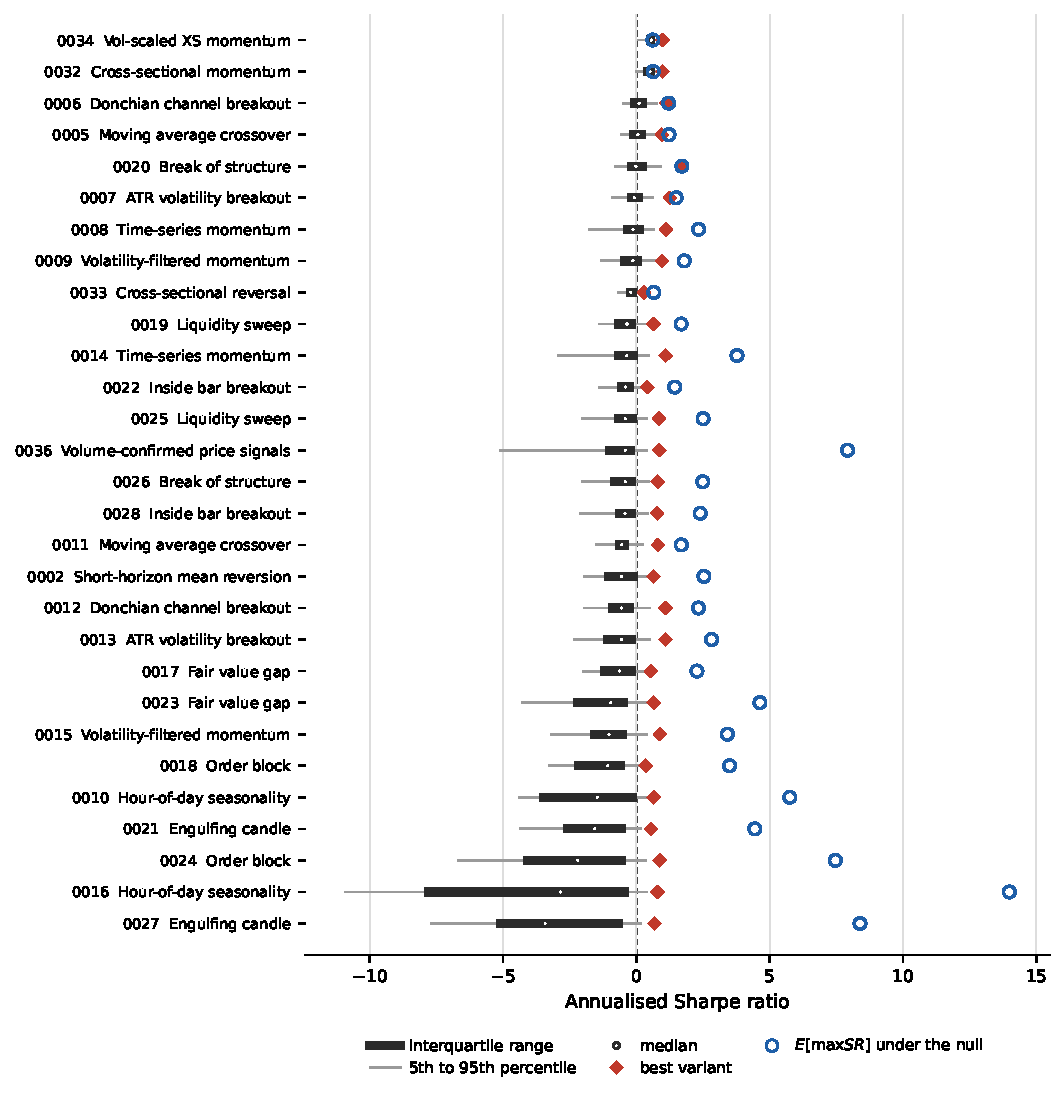
\includegraphics[width=\textwidth]{fig1.pdf}
\caption{Distribution of annualised Sharpe ratios across variants, one row
per scored sweep, ordered by median. Thick bar: interquartile range. Thin
line: 5th to 95th percentile. Red diamond: best variant. Open blue circle:
$E[\max SR]$ under the null. Where the circle lies to the right of the
diamond, the family underperformed chance.}
\label{fig:dist}
\end{figure}

The obvious explanation is transaction cost, and for some families that is
correct. But the diagnostics reported in \S\ref{sec:cost} show it is the
minority case: for seventeen of the twenty-nine sweeps with a cost decomposition,
the median variant is unprofitable \emph{before} any cost is charged. These
rules do not merely fail to overcome friction. They carry predictive content
pointing the wrong way.

\subsection{A joint test}

Twenty-nine separate tests, none of which rejects, is a weak statement. The
sweeps can instead be treated as one sample. Under the null that no family
carries an effect, the best variant of a sweep should fall above or below
$E[\max SR]$ with roughly equal probability, since $E[\max SR]$ approximates
the centre of the distribution of the maximum. Observing 27 of 29 on one side
has a two-sided binomial probability of $1.6 \times 10^{-6}$.

The direction matters. This is not a rejection in favour of the strategies; it
is a rejection against them. The median ratio of best variant to chance
expectation is 0.321, meaning the typical family's best member reached only a
third of what an equal number of coin flips would have produced.

The joint test is worth stating precisely because it sidesteps the detection
limit that weakens each sweep individually. No single sweep had the power to
distinguish a modest effect from zero. The collection has ample power to
distinguish ``these families are slightly better than chance'' from ``these
families are substantially worse than chance'', and it selects the latter.

Two caveats. The approximation $P(\text{best} < E[\max SR]) = 0.5$ under the
null is exact only for a symmetric distribution of the maximum, which is not
guaranteed; the true null probability is somewhat above 0.5, which makes the
test conservative in the direction reported. And the sweeps are not fully
independent: twelve families were run on both markets, and the crypto and
FX samples overlap in time. The effective sample is therefore smaller than 29,
though not by enough to overturn a $p$-value of this magnitude.

\subsection{Cost sensitivity}
\label{sec:cost}

Because gross and net returns were both recorded, the cost assumption can be
examined without re-running anything. Table~\ref{tab:cost} reports, for each sweep, the
median variant's annualised Sharpe gross of cost and net at the cost actually
charged, together with the breakeven cost.

Only measured points are tabulated. An earlier draft reported a grid of 0, 2,
6, 10 and 20 basis points, obtained by assuming Sharpe falls linearly in the
per-unit cost and interpolating from the two measured values. That assumption
is wrong. Mean return is linear in cost, but the standard deviation of the net
series is not, because per-bar cost scales with per-bar turnover, which varies
across the sample; for SW-0041 the 5th and 95th percentiles of turnover per
bar are 0.012 and 0.112, roughly a ninefold spread. Only the two endpoints
were ever computed from returns, so the three intermediate columns were
published numbers that had not been measured. They are removed.

Breakeven is defined as the per-variant round-trip cost at which that
variant's mean gross return reaches zero; the figure reported is the median
\emph{of those breakeven points}, which is not in general the breakeven of the
median variant. Earlier text described it as the latter.

The decomposition splits the registry cleanly:

\begin{itemize}
\item \textbf{Twelve sweeps have a positive median gross Sharpe}, and eight of
      the twelve are killed by friction. Donchian breakout and moving-average crossover on crypto
      are the only two single-asset sweeps whose breakeven cost (8.6 and 7.9~bps)
      exceeds the 6~bps charged, and whose median variant therefore remains
      positive after costs. The two cross-sectional momentum sweeps clear their
      higher charge by a wider margin (29.0 and 30.7~bps against 10), which is
      the subject of \S\ref{sec:best}.
\item \textbf{Seventeen sweeps have a negative median gross Sharpe.} No cost
      assumption rescues them. Inside bar breakout on crypto is the extreme
      case: a breakeven cost of $-15.2$~bps, meaning the median variant loses
      money even if the venue paid it 15~bps per round trip to trade.
\end{itemize}

The median breakeven across all twenty-nine is $-0.03$~bps. This is the single
most useful number for a practitioner reading this paper, and it is only
available because the gross series was retained.

The cost decomposition now covers all 29 scored sweeps. The three cross-sectional records that previously lacked one were voided and re-run as SW-0039, SW-0040 and SW-0041 with diagnostics enabled; their breakeven figures, 29.00 and 30.68~bps for the two momentum sweeps, are the highest in the registry and are discussed in \S\ref{sec:best}.

\subsection{Calibration of the power analysis}

Every pre-registration assumed a kurtosis of 8.0 and a skewness of $-0.2$ when
computing its detection limit. These were not arbitrary: 8.0 is a reasonable
figure for hourly returns on a liquid asset, and the planning assumptions were
frozen before any data was loaded, which is the point.

They were wrong in every sweep, in the same direction, by a large margin.

\begin{table}[ht]
\centering
\small
\begin{tabular}{lrr}
\toprule
& Assumed & Measured (median) \\
\midrule
Kurtosis & 8.0 & 2{,}835.3 \\
Skewness & $-0.2$ & 28.9 \\
\midrule
Sweeps where measured kurtosis exceeded assumed & \multicolumn{2}{r}{29 of 29} \\
Median underestimation factor & \multicolumn{2}{r}{354$\times$} \\
Maximum underestimation factor & \multicolumn{2}{r}{2{,}666$\times$} \\
\bottomrule
\end{tabular}
\caption{Planning assumptions against realised moments.}
\end{table}

The gap is not a defect in the assumption so much as a property of strategy
returns that is easy to overlook. The assumed figure describes the
\emph{asset}; the realised figure describes the \emph{strategy's return
series}, which is the asset return multiplied by a position that is frequently
zero and occasionally large. The skewness figure moves in the opposite direction to the assumption rather
than merely exceeding it: $-0.2$ was assumed, and the median realised value is
$+28.9$, positive in 27 of 29 sweeps. The two quantities move together --- the
sweeps with the largest skewness are the sweeps with the largest kurtosis
(SW-0010 at 128.5 and 17{,}961; SW-0027 at 123.3 and 19{,}466) --- which is
what a return series of mostly zeros punctuated by rare large moves produces.
The sign of the assumption was taken from asset returns, where negative
skewness is typical; it does not carry over to the conditioned series.

Conditioning on a trading rule concentrates the
distribution's mass at zero and leaves the tails intact, and kurtosis responds
to exactly that shape.

The practical implication is that power analyses for strategy sweeps that
plug in asset-level moments will understate the detection limit, in this
sample by a median factor of 354 in kurtosis and correspondingly in the
derived threshold. This is a correctable mistake, and it is correctable only
if someone reports both numbers.

\subsection{What actually drives the Deflated Sharpe Ratio}

The previous result has a consequence that is uncomfortable for the metric
this paper uses as its primary criterion.

\begin{table}[ht]
\centering
\small
\begin{tabular}{lr}
\toprule
Spearman correlation & $\rho$ \\
\midrule
Measured kurtosis vs.\ DSR & $-0.728$ \\
Best variant Sharpe vs.\ DSR & $+0.491$ \\
Measured kurtosis vs.\ $E[\max SR]$ & $+0.565$ \\
Mean exposure vs.\ measured kurtosis & $-0.194$ \\
\bottomrule
\end{tabular}
\caption{Rank correlations across the 29 scored sweeps.}
\end{table}

Across these sweeps, the Deflated Sharpe Ratio is more strongly associated
with the kurtosis of the return series than with how well the best strategy
performed. The path is visible in the third row: high kurtosis inflates
$E[\max SR]$, and an inflated null threshold drives the DSR toward zero
regardless of what the best variant achieved.

Splitting at a kurtosis of 200 makes the size of the effect concrete:

\begin{table}[ht]
\centering
\small
\begin{tabular}{lrrrr}
\toprule
& $n$ & Median DSR & Median $E[\max SR]$ & Median best \\
\midrule
Kurtosis $< 200$ & 8 & 0.122 & 1.70 & 1.037 \\
Kurtosis $\geq 200$ & 21 & 0.000 & 2.53 & 0.779 \\
\bottomrule
\end{tabular}
\caption{The DSR gap between the two groups is far larger than the gap in
underlying performance.}
\end{table}

The best variants of the two groups differ by 0.26 in annualised Sharpe. Their
chance thresholds differ by half again, and their Deflated
Sharpe Ratios differ by the entire available range. A reader comparing two
published DSR figures is, on this evidence, comparing the tail behaviour of
two return series at least as much as the quality of two strategies.

This should not be read as a claim that the Deflated Sharpe Ratio is wrong.
The non-normality adjustment it applies is correct, and a strategy whose
returns are a long series of zeros punctuated by rare large moves genuinely
does have a noisier maximum than one with well-behaved returns. The point is
narrower: the magnitude of that adjustment in realistic strategy data is large
enough to dominate the comparison, and a DSR reported without the
accompanying kurtosis is not interpretable.

Three limits on this finding. It is a correlation over 29 observations.
Strategy families differ simultaneously in kurtosis and in quality, and this
sample cannot separate the two. And an obvious candidate mechanism --- that
sparse, infrequently-held positions produce both the high kurtosis and the
poor performance --- is not supported: mean exposure and kurtosis are
essentially uncorrelated ($\rho = -0.19$).

\subsection{Overfitting probability}

Reporting PBO for every sweep rather than only the best one produces a
pattern worth stating explicitly. The median PBO across the 29 sweeps is
0.188, which is low. Taken at face value this says the variant ranking is
usually stable out of sample.

That is true, and it is not good news for the strategies. When a family is
reliably unprofitable, the ranking within it is stable precisely because the
ordering is driven by a real and persistent quantity --- turnover cost ---
rather than by noise. Hour-of-day seasonality scores a PBO of exactly 0.000
on both markets: the worst variants stay worst. Low PBO is informative about
whether a selection procedure generalises, not about whether the thing
selected is worth holding.

The highest PBO figures appear where they should: liquidity sweep on FX at
0.573, volatility-scaled cross-sectional momentum at 0.399, cross-sectional
momentum at 0.339. These are the sweeps whose top variants are closest to
being interesting, and they are also the sweeps where selecting the top
variant is closest to a coin flip.

\subsection{The best result in the registry}
\label{sec:best}

The strongest sweep, SW-0041, tests volatility-scaled cross-sectional
momentum on a point-in-time top-20 crypto universe: assets ranked by trailing
return divided by trailing volatility rather than by raw return, 45 fully
enumerated variants over 56{,}126 hourly observations. It supersedes SW-0034,
voided as described in \S\ref{sec:corrections}.

\begin{table}[ht]
\centering
\small
\begin{tabular}{lr}
\toprule
Best annualised Sharpe, net & 1.0431 \\
$E[\max SR]$ under the null & 0.7744 \\
Critical Sharpe at the threshold & 1.4528 \\
Deflated Sharpe Ratio & 0.745 \\
Probability of Backtest Overfitting & 0.399 \\
Minimum detectable Sharpe (realised) & 1.804 \\
\midrule
Gross Sharpe: mean / median / max & 0.823 / 0.814 / 1.529 \\
Share of variants with positive gross Sharpe & 100\% \\
Share with positive net Sharpe & 86.7\% \\
Median breakeven cost & 30.68 bps \\
Cost charged & 10.0 bps \\
\midrule
Mean gross exposure & 1.988 \\
Mean directional tilt & $-0.0000$ \\
Mean market beta & $+0.027$ \\
Market-neutral residual Sharpe, mean & 0.812 \\
\midrule
Residual Sharpe on shuffled panels & $-0.079 \pm 0.491$ \\
Observed residual Sharpe & $+0.812$ \\
$z$ against the shuffled null & 1.816 \\
\bottomrule
\end{tabular}
\caption{SW-0041 in full. Verdict: no edge found.}
\end{table}

This sweep is the one case in the registry where the surface statistics look
like an effect, and it is worth setting out exactly what they show and what
they do not.

Every one of the 45 variants has positive gross Sharpe, with a mean of 0.823.
The portfolio is genuinely dollar-neutral --- mean directional tilt is zero to
four decimal places and mean market beta is $+0.027$ against an equal-weighted
index of the investable universe --- so this is not the market trend
reappearing in another form, which is the failure mode that contaminated the
voided predecessor. The market-neutral residual Sharpe, 0.812, is almost
identical to the raw gross figure. The median variant breaks even at 30.68
basis points of round-trip cost against the 10 charged, so the effect is not
one that only exists at zero cost. Cross-sectional momentum (SW-0039) shows
the same pattern at slightly lower magnitude: 100\% positive gross Sharpe,
median breakeven 29.00~bps, mean beta $-0.096$.

Two independent criteria nevertheless place this inside the noise.

The first is the pre-registered one. The best net Sharpe, 1.043, falls short
of the 1.453 required to clear a Deflated Sharpe Ratio of 0.95 given 45
trials and the realised moments. The PBO of 0.399 says the same thing from a
different direction: the variant that ranks best in a training split lands
below the out-of-sample median in 40\% of the 12{,}870 splits.

The second was computed after the fact and is reported as exploratory. Each
asset's returns were shuffled independently, destroying both serial and
cross-sectional structure while preserving every per-asset return
distribution, and the whole sweep re-run on ten such panels. The mean residual
Sharpe across those panels was $-0.079$ with a standard deviation of 0.491.
The observed $+0.812$ sits 1.82 standard deviations above that, which is
inside the spread. For SW-0039 the equivalent figure is 0.81. The instrument
cannot separate this from a panel with no structure in it.

The gap between the two framings is the useful part. A reader shown only the
gross Sharpe distribution --- all 45 variants positive, breakeven at three
times the cost charged, beta of 0.03 --- would reasonably conclude that
something is there. A reader shown only the DSR would conclude nothing is.
Both were computed from the same returns. The pre-registered rule decides,
and it says no; the shuffled-panel calibration, which was not pre-registered,
happens to agree. This paper reports the disagreement rather than the figure
that reads better, which is the only reason the comparison is available at
all.

A holdout sweep over the same parameter space (SW-0035) was pre-registered
and timestamped before its window opened. It remains unrun, and its window
does not close until 2029. Running it early at reduced power would consume a
single-use test to obtain a result the power analysis already predicts would
be inconclusive.

\subsection{Detection limit}

The median minimum detectable annualised Sharpe across scored sweeps was 3.49.
This is high, and it is the most important caveat in the paper. A real effect
with a Sharpe of 0.8 --- which would be a good strategy --- sits well below
this threshold for most sweeps and would not have been detected.

The limit varies enormously across sweeps, from 1.80 for the cross-sectional
sweeps to 29.41 for hour-of-day seasonality on FX. The driver is the
dispersion of variant Sharpe ratios within the family: a family whose
variants range from $-17.6$ to $+0.8$ carries so much internal variance that
no realistic effect could be distinguished from it. Those sweeps are, in
practice, uninformative, and the appendix reports their detection limits so
that a reader can discount them rather than count them as evidence.

The correct reading of the headline result is therefore: \emph{within this
region, no effect large enough to clear the stated detection limit exists}.
Smaller effects are untested, not refuted.

\section{Corrections and integrity notes}
\label{sec:corrections}

\subsection{Six voided runs, in two waves}

Eight records in the registry are marked void. Six are the failed executions
below; the other two are the declined runs of \S5.2, voided for a different
reason.

\paragraph{First wave: an empty matrix scored as a null result.}
Three sweeps (SW-0029, SW-0030, SW-0031) produced returns matrices that were
identically zero. The sweep process had been killed by the operating system's
out-of-memory handler partway through, leaving the allocated matrix unwritten.
The scoring pipeline then accepted the empty matrix as a valid null result and
reported ``best Sharpe 0.0, zero variants positive'', with a Deflated Sharpe
Ratio of exactly 0.5. It was not a finding; it was a crashed run that
resembled one, which is the worst output this registry could produce. A guard
now refuses to score a matrix in which every variant has a Sharpe of exactly
zero. The three hypotheses were re-run as SW-0032, SW-0033 and SW-0034.

\paragraph{Second wave: a weight-allocation defect in the cross-sectional
engine.} Those replacements were themselves voided. An earlier draft of this
paper reported SW-0034 and SW-0032 as the two sweeps whose best variant
exceeded chance expectation, with Deflated Sharpe Ratios of 0.823 and 0.809.
A line-by-line audit of the execution engine, undertaken before submission,
found the following in the cross-sectional weight allocator: assets outside
the point-in-time investable universe were assigned a score of $-\infty$ and
therefore sorted to the \emph{front} of the ranking, so the short leg --- taken
from the front --- was allocated entirely to non-investable assets whose
returns are zeroed by construction. Half the variants in each sweep, the 45
long/short ones out of 90, held no short position at all. They were long-only
books at gross exposure 2.0 wearing the turnover cost of a short leg that did
not exist.

The diagnosis was confirmed rather than inferred. The stored returns matrices
reproduce to within $2.6\times10^{-8}$ under a replay of the defective
allocator and diverge materially under the corrected one, with per-variant
correlations of 0.54 to 0.69 between the two. The long-only branch was
untouched by the defect, but corrupted variants still enter the trial count,
the expected-maximum-Sharpe null and the CSCV combinatorics, so the primary
metric of all three sweeps was invalid.

The three were voided, the defect fixed, and a regression test added covering
universe containment, dollar neutrality, gross exposure and leg overlap. The
hypotheses were re-registered as SW-0039, SW-0040 and SW-0041, re-hashed,
re-anchored to the Bitcoin blockchain, and re-run. One deliberate change was
made to the search space and recorded in the new pre-registrations: the
long-only exit rule was removed, because a long-only book at gross exposure
2.0 does not test a cross-sectional hypothesis. That exclusion was decided
after seeing which branch had dominated the voided results and is marked as
such; it halves the variant count, which lowers the multiple-testing penalty
and makes the remaining test easier rather than harder to pass. The
replacements scored 0.605, 0.001 and 0.745.

The pre-registrations and Bitcoin timestamps of all six voided records remain
valid; only their execution failed. Both the voided records and their
replacements are public, with the reason and the superseding identifier on
each page.

\paragraph{A record that is not independent evidence.}
SW-0040 (cross-sectional reversal) is implemented as the negation of the
momentum score, so with a symmetric long/short fraction its portfolio is the
arithmetic inverse of SW-0039. Measured per-variant correlation between the
two returns matrices is $-0.997$ to $-0.999$, and their gross Sharpe, residual
Sharpe, turnover and breakeven figures are mirror images to four decimal
places. Only net Sharpe differs non-trivially, because transaction costs
subtract from both legs rather than reflecting. The two records are one piece
of evidence with a sign, not two, and both carry an annotation saying so. They
are counted separately in the sweep totals, which overstates the independent
evidence in the cross-sectional family by one sweep.

\subsection{Two declined runs}

SW-0003 tested short-horizon continuation on BTC and ETH as a follow-on to
SW-0002. Its discovery sample produced a best annualised Sharpe of 1.489
against $E[\max SR]$ of 2.068 and a DSR of 0.050. SW-0004, the holdout
reserved for it, was voided as declined rather than failed: a confirmatory
test on a hypothesis the discovery sample has already refuted adds no
information, and running it would only consume a sealed window. SW-0003 is
excluded from the 29 scored sweeps and from all totals reported here.

\subsection{Symbols counted as independent trials}

In the 26 multi-symbol sweeps --- 17{,}676 of the 17{,}811 scored variants, or
99\% of the registry --- a variant is one parameter combination applied to one
symbol, so the same combination run on BTCUSDT and on ETHUSDT counts as two
trials. SW-0008 is typical: 270 parameter combinations across two symbols are
enumerated and scored as 540 trials.

This affects the primary metric in two ways, both in the same direction.
The Deflated Sharpe Ratio penalises by trial count, so scoring 540 rather than
270 applies a heavier multiple-testing penalty than the number of distinct
hypotheses warrants. And $E[\max SR]$ assumes the trials are independent,
which paired symbols are not: the same rule on BTCUSDT and ETHUSDT produces
correlated return series, so the effective number of independent trials is
below the nominal count, and the null threshold is correspondingly higher than
an effective-$N$ calculation would give.

Both errors therefore run in the conservative direction: they make the
threshold harder to clear, not easier. This is the opposite of the bias
described in the next subsection, and it is reported for the same reason ---
a reader recomputing these figures with distinct parameter combinations as the
unit, or with an effective trial count, would obtain Deflated Sharpe Ratios
somewhat higher than those reported here. No sweep is close enough to the 0.95
threshold for this to change a verdict: the largest, SW-0041, is a
single-universe cross-sectional sweep with no symbol multiplication at all.

\subsection{Variants that never traded}

In seven of the 29 scored sweeps the number of variants scored is smaller
than the number enumerated, 17{,}811 against 18{,}630 in total. The difference consists
entirely of variants whose parameter combination produced no trade at all
over the sample: the Sharpe of an identically zero return series is
undefined, and such columns were excluded at scoring time.

The scoring pipeline flags this automatically. Every affected record carries
an integrity note of the form \emph{``Trial count differs from
pre-registration: declared 540, supplied 261. Explain this in the record.''},
and the explanation is recorded in that sweep's \texttt{annotations.json}.

The exclusion is not neutral. The Deflated Sharpe Ratio penalises by trial
count, so scoring 261 trials rather than the 540 enumerated applies a lighter
multiple-testing penalty and biases the DSR \emph{upward}. The error, in other
words, runs in the permissive direction. It is reported here for that reason
rather than despite it.

Its practical effect on the conclusions is nil. The largest DSR among the
seven affected sweeps is 0.002, and the two with the largest shortfall
(SW-0022 and SW-0028, inside bar breakout, 261 of 540 and 405 of 810) scored
0.002 and 0.00007. The two sweeps carrying the paper's highest scores,
SW-0039 and SW-0041, had no excluded variants: all 45 traded in each.

These corrections are reported because a registry that conceals its own
failed runs reproduces the problem it exists to address.

\section{What this study does not show}

\begin{enumerate}
\item \textbf{That technical trading does not work.} The tested region is
      small relative to the space of possible strategies. Nothing here
      addresses discretionary trading, execution-based strategies, alternative
      data, or any family not enumerated.

\item \textbf{That effects below the detection limit are absent.} With a
      median minimum detectable Sharpe of 3.49, this study is uninformative
      about modest but real edges.

\item \textbf{That the cost model is correct.} Costs were fixed in advance,
      which prevents tuning, but a wrong fixed assumption is still wrong. The
      direction matters: if real costs are lower than assumed, some families
      would score better.

\item \textbf{Generality across timeframes.} All sweeps use hourly bars.
      Higher-frequency effects are outside scope entirely.

\item \textbf{Generality across venues or instruments.} Cryptocurrency data
      comes from a single exchange archive, and the single-asset sweeps use
      two crypto symbols and three FX pairs. Cross-venue differences are not
      examined.

\item \textbf{Freedom from survivorship bias in every sweep.} Point-in-time
      universe construction was applied to the cross-sectional sweeps. The
      fixed-symbol sweeps use symbols that still trade today, which for BTC,
      ETH and the three FX majors is a mild assumption but not a vacuous one.
\end{enumerate}

\section{Reproduction}

The registry --- every pre-registration, its canonical frozen form, its
SHA-256 hash, its OpenTimestamps proof, the scoring output, the diagnostics
and the annotations --- is at
\url{https://github.com/mobinmoharami/sweep-registry}. Data are downloadable
from Binance public archives with the included scripts; no API key or account
is required.

The returns matrices themselves are not in the repository. They total 4.5~GB,
which exceeds both the per-file and per-repository limits of the hosting
service; the largest single matrix is 444~MB. What is published instead is
\texttt{RETURNS\_CHECKSUMS.json}, giving the SHA-256 of every matrix, together
with the scripts that regenerate them. A third party who re-runs a sweep can
confirm bit-for-bit that the matrix scored here is the matrix their run
produced:

\begin{verbatim}
python run_sweep.py sweeps/SW-0008
sha256sum sweeps/SW-0008/returns.npy    # compare to RETURNS_CHECKSUMS.json
python finalize.py sweeps/SW-0008
\end{verbatim}

This is weaker than publishing the matrices directly, and the author intends
to deposit them with a data repository that accepts archives of this size.

Every number, table and figure in this paper is regenerated from the registry
by \texttt{paper/analysis.py}, which reads the sweep directories and
hard-codes nothing. Running it writes \texttt{paper/build/stats.txt}, in which
each figure quoted here appears with its label; any discrepancy between that
file and this text is a defect in the text.

To verify that a pre-registration predates its result, recompute the SHA-256
of the frozen document and check it against the \texttt{.ots} proof with the
OpenTimestamps client. The proof resolves to a Bitcoin block height and
timestamp. The chain view recomputes every hash from the frozen documents on
request, so a record altered after sealing reports as broken rather than
continuing to display a stale verification badge.

\section{Conclusion}

Seventeen strategy families, enumerated into 18{,}630 variants across two
asset classes and up to eight years of hourly data, produced nothing above a
Deflated Sharpe Ratio of 0.745 against a pre-specified threshold of 0.95. In
27 of 29 scored sweeps the best variant performed worse than chance
expectation, and the single strongest result carries a Probability of
Backtest Overfitting of 0.40.

Three findings survive independently of whether anyone cares about these
particular families. A sign test across sweeps rejects the joint null against
the strategies at $p = 1.6\times10^{-6}$, which no individual sweep had the
power to do. A cost decomposition shows that most of these families are
unprofitable before friction rather than because of it. And the moments
assumed in every power analysis were wrong in the same direction in every
sweep, by a median factor of 354, with the consequence that the Deflated
Sharpe Ratio in this sample tracks kurtosis more closely than performance.

The methodological claim is narrower and more durable than the empirical one:
pre-registration with cryptographic timestamping is cheap, it is practical for
an individual researcher rather than only for institutions, and publishing the
full distribution of a negative sweep costs nothing while being worth more
than another positive result of unknown provenance.

\section*{Disclosure}

The author used an AI assistant for drafting and editing this manuscript. All
data collection, code, analysis and conclusions are the author's own, and the
author takes full responsibility for the content.

\section*{Data and code availability}

All materials are public at
\url{https://github.com/mobinmoharami/sweep-registry} under the terms stated
in that repository.

\appendix

\section{All scored sweeps}

\footnotesize
\setlength{\tabcolsep}{3.4pt}
\begin{longtable}{llrrrrrrrr}
\caption{Every scored sweep. Declared is the enumerated grid; scored excludes
variants that never traded. Best and $E[\max SR]$ are annualised Sharpe
ratios; MDS is the minimum detectable annualised Sharpe at 80\% power;
PBO is the probability of backtest overfitting.}\\
\toprule
ID & Family & Market & Decl. & Scored & Best & $E[\max]$ & DSR & MDS & PBO \\
\midrule
\endfirsthead
\toprule
ID & Family & Market & Decl. & Scored & Best & $E[\max]$ & DSR & MDS & PBO \\
\midrule
\endhead
\bottomrule
\endfoot
\input{tableA1}
\end{longtable}
\normalsize

\section{Cost sensitivity}

\small
\begin{longtable}{lrrrr}
\caption{Median variant annualised Sharpe, gross and net at the cost charged,
by sweep. Both columns are measured; no values are interpolated. Breakeven is
the median of the per-variant round-trip costs at which mean gross return
reaches zero; negative means no cost level makes that variant profitable. All
29 scored sweeps carry diagnostics.\label{tab:cost}}\\
\toprule
ID & Gross & Cost (bps) & Net & Breakeven \\
\midrule
\endfirsthead
\toprule
ID & Gross & Cost (bps) & Net & Breakeven \\
\midrule
\endhead
\bottomrule
\endfoot
\input{tableA3}
\end{longtable}
\normalsize

\section{Variant distributions}

\small
\begin{longtable}{lrrrrrrrr}
\caption{Annualised Sharpe distribution across variants within each sweep.
Pos.\ is the share of variants with positive Sharpe.}\\
\toprule
ID & Min & P05 & P25 & Median & P75 & P95 & Max & Pos. \\
\midrule
\endfirsthead
\toprule
ID & Min & P05 & P25 & Median & P75 & P95 & Max & Pos. \\
\midrule
\endhead
\bottomrule
\endfoot
\input{tableA2}
\end{longtable}

\begin{thebibliography}{9}

\bibitem[Ammann et al.(2022)]{ammann2022}
Ammann, M., Burdorf, T., Liebi, L., St\"ockl, S. (2022).
\emph{Survivorship Bias in Cryptocurrency Data}. SSRN 4287573.

\bibitem[Bailey and L\'opez de Prado(2014)]{bailey2014}
Bailey, D.~H., L\'opez de Prado, M. (2014).
The Deflated Sharpe Ratio: Correcting for Selection Bias, Backtest
Overfitting and Non-Normality.
\emph{Journal of Portfolio Management} 40(5), 94--107.

\bibitem[Bailey et al.(2017)]{bailey2017}
Bailey, D.~H., Borwein, J., L\'opez de Prado, M., Zhu, Q.~J. (2017).
The Probability of Backtest Overfitting.
\emph{Journal of Computational Finance} 20(4), 39--69.

\bibitem[Harvey et al.(2016)]{harvey2016}
Harvey, C.~R., Liu, Y., Zhu, H. (2016).
$\ldots$ and the Cross-Section of Expected Returns.
\emph{Review of Financial Studies} 29(1), 5--68.

\bibitem[L\'opez de Prado(2018)]{lopezdeprado2018}
L\'opez de Prado, M. (2018).
\emph{Advances in Financial Machine Learning}. Wiley.

\bibitem[Todd(2016)]{ots}
Todd, P. (2016). \emph{OpenTimestamps: Scalable, Trustless, Distributed
Timestamping with Bitcoin}. \url{https://opentimestamps.org}

\end{thebibliography}

\end{document}
